

\begin{figure}[h!]
\centering
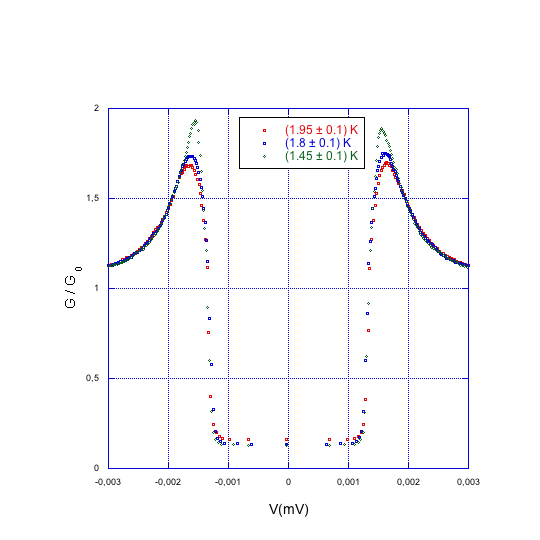
\includegraphics[scale=0.45]{graph1}
\caption{Hola\label{gv_3}}
\end{figure}

\begin{figure}[h!]
\centering
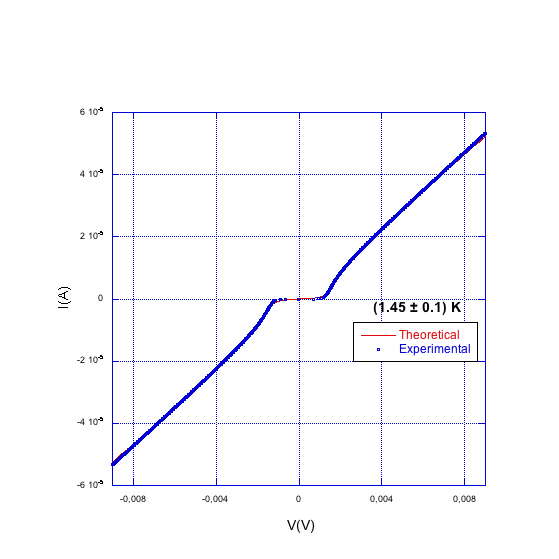
\includegraphics[scale=0.45]{graph2}
\caption{Hola\label{iv_theo_exp}}
\end{figure}

\begin{figure}[h!]
\centering
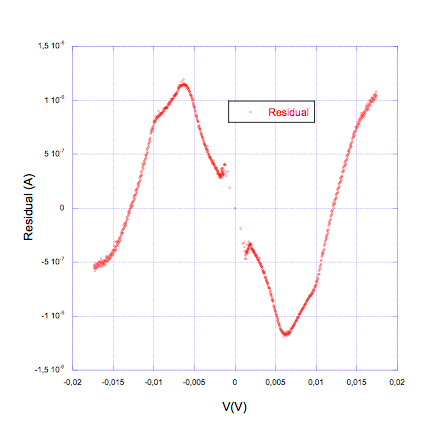
\includegraphics[scale=0.45]{graph3}
\caption{Hola\label{graph3}}
\end{figure}

\begin{figure}[h!]
\centering
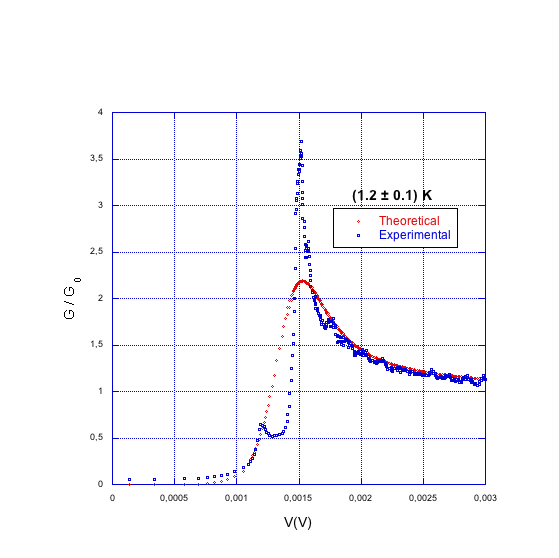
\includegraphics[scale=0.4]{graph4}
\caption{Hola\label{graph4}}
\end{figure}

\begin{figure}[h!]
\centering
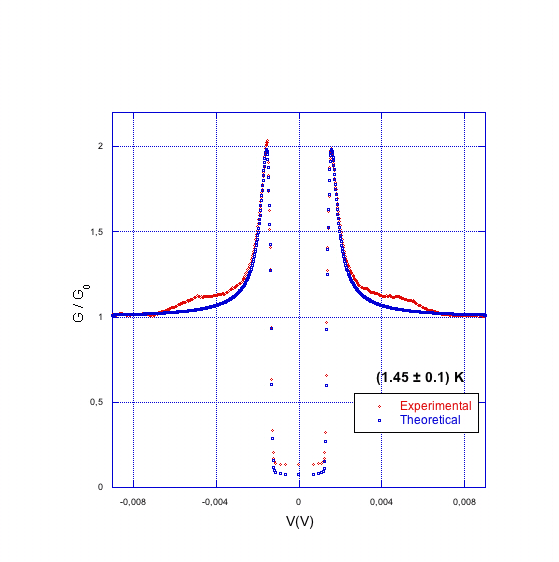
\includegraphics[scale=0.4]{graph5}
\caption{Hola\label{graph5}}
\end{figure}

\begin{figure}[h!]
\centering
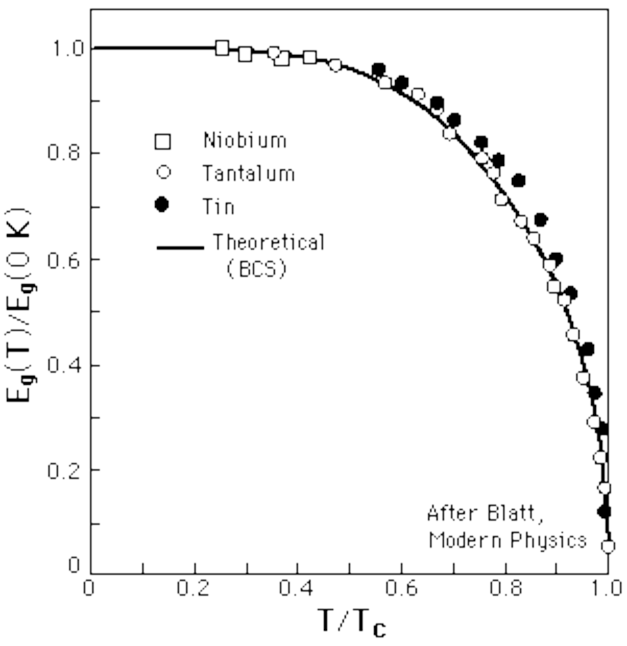
\includegraphics[scale=0.6]{bcs_gap2}
\caption{\small Reduced values of the observed energy gap as a function of the reduced temperature, after Towsend and Sutton. The solid curve is drawn for the BCS theory. \label{bcs_gap}}
\end{figure}


\begin{figure}
\centering
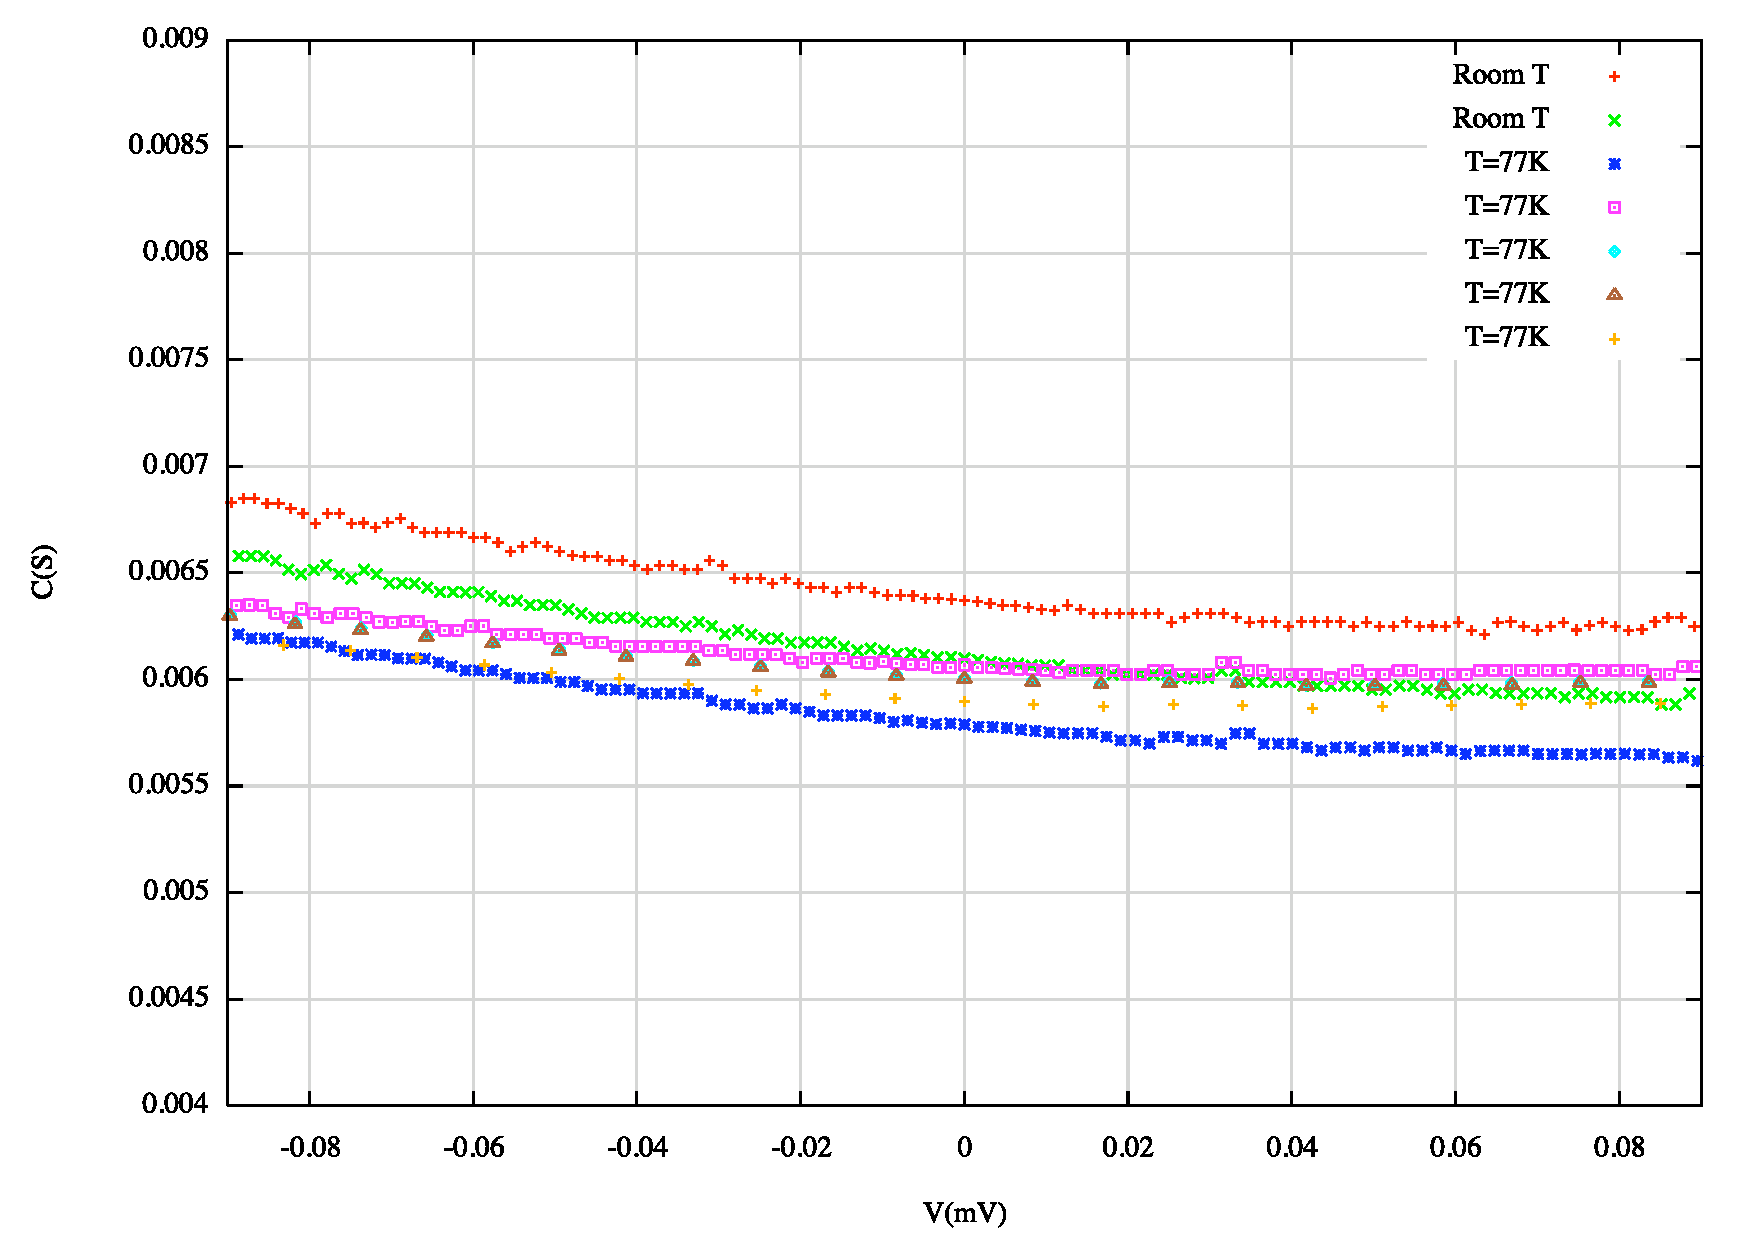
\includegraphics[scale=0.6]{conductance}
\caption{\small Conductance curves . \label{conductance}}
\end{figure}



\subsection{Energy gap}
We have measured the lead's energy gap as $(1.4 \pm 0.1)meV$ below $4.2K$. The BCS theory predicts a temperature dependance, nevertheless in the range we have measured it, i.e. below the helium vaporization and above the Aluminum critical temperatures, this variation is less than the experimental error. This can be seen in fig.\ref{bcs_gap}.

The data almost agree with BCS theory. In fig.\ref{iv_theo_exp} can be seen the I-V curve, which is modified near the gap when the temperature is below the $T_c$. The experimental and theoretical data are difficult to distinguish. 

However, 



1) Symmetric?

2) Al a little bit superconducting

3) Phonons

4)  How have been made the graphs... smoothing... effects below the smoothing cannot be considered.

5) Tc for films is greater than the bulk Tc's... So at 1.2K is possible that some parts of the Al film are superconductors. In this case, we have normal-super and super-super junctions added in parallel.



